%-----------------------------------------------------------------------------%
\chapter{\babDua}
\label{bab:2}
%-----------------------------------------------------------------------------%
Untuk memulai penelitian, dibutuhkan kerangka berpikir yang sesuai untuk permasalahan yang ingin dipecahkan. Untuk membentuk kerangka berpikir yang sesuai, perlu dikaitkan dengan hasil studi literatur yang telah dilakukan. Oleh karena itu, pada bab ini, akan dijelaskan hasil studi literatur yang telah dilakukan yang telah dikaitan dengan kerangka kerja untuk penelitian ini.


%-----------------------------------------------------------------------------%
\section{Cubic Splines}
\label{sec:cubicSplines}
%-----------------------------------------------------------------------------%
\f{Splines} merupakan salah satu pendekatan dalam permasalahan interpolasi. Berbeda dengan interpolasi polinomial yang hanya menggunakan satu fungsi polinomial untuk memenuhi semua \f{data points}, \f{Splines} menggunakan beberapa fungsi polinomial derajat rendah untuk melewati semua titik-titik pada data.
Diketahui data sebanyak $n$ yang merupakan koordinat titik dengan format $(x_1, y_1), (x_2, y_2), ..., (x_n, y_n)$ dengan syarat $x_i$ bersifat \f{distinct} dan terurut secara \f{ascending}. Sebuah \bo{Cubic Splines} $S(x)$ melewati titik $(x_1, y_1), (x_2, y_2), ..., (x_n, y_n)$ merupakan sebuah himpunan/\f{set} dari polinomial pangkat tiga:
\begin{center}
	\[ S_{1}(x) = y_1 + b_1(x - x_1) + c_1(x - x_1)^2 + d_1(x - x_1)^3 \text{  pada interval  } [x_1, x_2] \]
	\[ S_{2}(x) = y_1 + b_1(x - x_2) + c_1(x - x_2)^2 + d_1(x - x_2)^3 \text{  pada interval  } [x_1, x_2] \]
	\vdots
	\[ S_{n-1}(x) = y_{n-1} + b_{n-1}(x - x_{n-1}) + c_{n-1}(x - x_{n-1})^2 + d_{n-1}(x - x_{n-1})^3 \text{  pada interval  } [x_{n-1}, x_n]\]
\end{center}

Sebuah \bo{Cubic Splines} $S(x)$ memiliki beberapa properti antara lain:
\begin{itemize}
	\item Properti 1: \[ S_{i}(x_i) = y_i  \text{  and  }  S_{i}(x{i}+1) = y_{i+1} \] Properti ini menjamin \(S(x)\) sukses menginterpolasi titik-titik yang diberikan.
	\item Properti 2: \[ S'_{i-1}(x_i) = S'_{i}(x_1) \text{  for  } i=2,...,n-1 \] Properti ini mengakibatkan \f{slopes} dari dua bagian spline yang berbeda dapat bertemu pada suatu tempat.
	\item Properti 3: \[ S''_{i-1}(x_i) = S''_{i}(x_1) \text{  for  } i=2,...,n-1 \] Properti ini menjamin \f{curvature} menjadi \f{smooth}
\end{itemize}

Mendefinisikan \f{spline} dari suatu himpunan titik-titik data merupakan kegiatan mencari koefisien dari $b_i, c_i, d_i$ yang menyebabkan properti 1,2, dan 3 terpenuhi. Terdapat beberapa properti tambahan yang digunakan agar hasil komputasi menjadi lebih simpel dan hasil yang diberikan lebih deskriptif. Properti ini disebut dengan \f{endpoints}. \f{Endpoints} yang digunakan dapat dipilih satu dari beberapa varian di bawah ini:
\begin{itemize}
	\item Properti 4a \bo{Natural spline} : \[ S''(x) = 0 \text{  dan  } S''_{n-1}(X_n) = 0\]
	\item Properti 4b \bo{Curvature-adjusted cubic spline} : \[ S''_{1}(x_1) \text{  dan  }  S''{n-1}(x_n) \text{ assign ke sebuah nilai arbitrary}\]
	\item Properti 4c \bo{Clamped cubic spline} : \[ S'_{1}(x_1) \text{  dan  } S'_{n-1}(x_n) \text{  assign ke sebuah nilai arbitrary}\]
	\item Properti 4d \bo{Parabolically terminated cubic spline} : \[  S_{1} \text{ dan } S_{n-1} \text{ merupakan polinomial derajat kurang dari atau sama dengan 2}\]
	\item Properti 4e \bo{Not-a-knot cubic spline} :\[ S'''_{1}(x_2) = S'''_{2}(x_2) \text{  dan  } S'''_{n-2}(x_{n-1}) = S'''_{n-1}(x_{n-1}) \]
\end{itemize}

Dengan adanya properti \f{endpoints} di atas, jumlah persamaan yang perlu diselesaikan untuk menemukan solusi interpolasi yaitu sebanyak $3n-3$.
Implikasi yang dihasilkan oleh properti-properti spline dengan jumlah persamaan yang ada adalah sebagai berikut:
\begin{itemize}
	\item Properti 1 mengimplikasikan \(n-1\) persamaan : \[ y_2 = S_{1}(x_2) = y_1 + b_1(x - x_1) + c_1(x - x_1)^2 + d_1(x - x_1)^3 \]  \vdots \begin{equation} \label{eq:2.1} y_n =  S_{n-1}(x_n) = y_{n-1} + b_{n-1}(x_n - x_{n-1}) + c_{n-1}(x_n - x_{n-1})^2 + d_{n-1}(x_n - x_{n-1})^3 \end{equation}
	\item Properti 2 mengimplikasikan \(n-2\) persamaan : \[ 0 = S'_{1}(x_2) - S'_{2}(x_2) = b_1 + 2c_1(x_2 - x_1) + 3d_1(x_2 - x_1)^2 - b_2 \] \vdots \begin{equation} \label{eq:2.2}  0 = S'_{n-2}(x_{n-1}) - S'_{n-1}(x_{n-1}) = b_{n-2} + 2c_{n-2}(x_{n-1} - x_{n-2}) + 3d_{n-2}(x_{n-1} - x_{n-2})^2 - b_{n-1}  \end{equation}
	\item Properti 3 mengimpliaksikan \(n-2\) persamaan : \[ 0 = S''_{1}(x_2) - S''{2}(x_2) = 2c_1 + 6d_1(x_2 - x_1) - 2c_2 \] \vdots \begin{equation} \label{eq:2.3}  0 = S''_{n-2}(x_{n-1}) - S''{n-1}(x_{n-1}) = 2c_{n-2} + 6d_{n-2}(x_{n-1} - x_{n-2}) - 2c_{n-1}  \end{equation}
\end{itemize}

Menyelesaikan persamaan-persamaan di atas dapat dilakukan dengan cara mengubahnya ke bentuk yang lebih simpel. Oleh karena itu, diperlukan beberapa notasi tambahan baru:
\begin{equation} \label{eq:2.4}  c_n = S''_{n-1}(x_n) / 2  \end{equation}
\begin{equation} \label{eq:2.5} \delta_{i} = x_{i+1} - x_i \end{equation}
\begin{equation} \label{eq:2.6} \Delta_{i} = y_{i+1} - y_i \end{equation}

Selesaikan persamaan \equ~(\ref{eq:2.3}):
\begin{equation} \label{eq:2.7}
	d_i = \frac{ c_{i+1} - c_i }{ 3\delta-{i} } \text{   for } i=1,2,...,n-1
\end{equation}

Selesaikan persamaan \equ~(\ref{eq:2.1}) dengan substitusi \equ~(\ref{eq:2.7})
\begin{equation} \label{eq:2.8}
	\begin{split}
		b_i &=  \frac{\Delta_i}{\delta_i} - c_{i}d{i} - d_{i}\delta^2_{i} \\
		&= \frac{\Delta_i}{\delta_i} - c_{i}d{i} - \frac{\delta_i}{3}(c_{i+1} - c_i) \\
		&= \frac{\Delta_i}{\delta_i} - \frac{\delta_i}{3}(2c_i + c_{i+1}) \text{   for } i = 1,2...,n-1
	\end{split}
\end{equation}

Selesaikan persamaan \equ~(\ref{eq:2.2}) dengan substitusi \equ~(\ref{eq:2.7}) dan \equ~(\ref{eq:2.7})
\begin{equation} \label{eq:2.9}
	\delta_{n-2}c_{n-2} + 2(\delta_{n-2} + \delta_{n-1})c_{n-1} + \delta_{n-1}c_n = 3(\frac{\Delta_{n-1}}{\delta_{n-1}} - \frac{\Delta_{n-2}}{\delta_{n-2}})
\end{equation}

Dan juga dua buah persamaan \f{endpoints} (untuk kasus ini menggunakan \f{natural spline}):
$$ S''_{1}(x_1) = 0 \Rightarrow 2c_1 = 0 $$
$$ S''_{n-1}(x_n) = 0 \Rightarrow 2c_n = 0 $$

Dengan demikian, hal ini akan memberikan $n$ persamaan dalam $n$ buah nilai $c_i$ yang dapat dikonstruksi sebagai perkalian matriks:
\begin{equation} \label{eq:2.10}
	\begin{bmatrix}
		1        & 0                     & 0                     &              &                               &             \\
		\delta_1 & 2\delta_1 + 2\delta_2 & \delta_2              &              &                               &             \\
		0        & \delta_2              & 2\delta_2 + 2\delta_3 & \delta_3     &                               &             \\
		         & \ddots                & \ddots                & \ddots       & \ddots                        &             \\
		         &                       &                       & \delta_{n-2} & 2\delta_{n-2} + 2\delta_{n-1} & \delta{n-1} \\
		         &                       &                       & 0            & 0                             & 1           \\
	\end{bmatrix}
	\times
	\begin{bmatrix}
		c_1    \\
		c_2    \\
		\\
		\vdots \\
		\\
		c_n    \\
	\end{bmatrix}
	=
	\begin{bmatrix}
		0                                                                        \\
		3(\frac{\Delta_2}{\delta_2} - \frac{\Delta_1}{\delta_1})                 \\
		\\
		\vdots                                                                   \\
		3(\frac{\Delta_{n-1}}{\delta_{n-1}} - \frac{\Delta_{n-2}}{\delta_{n-2}}) \\
		0                                                                        \\
	\end{bmatrix}
\end{equation}
% %-----------------------------------------------------------------------------%
% \section{Apa itu \latex?}
% \label{sec:latex}
% %-----------------------------------------------------------------------------%

% %-----------------------------------------------------------------------------%
% \subsection{\latex~Secara Singkat}
% \label{sec:latexBrief}
% %-----------------------------------------------------------------------------%
% Berdasarkan \cite{latex:intro}: \\
% \begin{tabular}{| p{13cm} |}
% 	\hline
% 	\\
% 	LaTeX is a family of programs designed to produce publication-quality typeset documents. It is particularly strong when working with mathematical symbols.                                                                                                                                                                                                                                      \\
% 	The history of LaTeX begins with a program called TEX. In 1978, a computer scientist by the name of Donald Knuth grew frustrated with the mistakes that his publishers made in typesetting his work. He decided to create a typesetting program that everyone could easily use to typeset documents, particularly those that include formulae, and made it freely available. The result is TEX. \\
% 	Knuth's product is an immensely powerful program, but one that does focus very much on small details. A mathematician and computer scientist by the name of Leslie Lamport wrote a variant of TEX called  that focuses on document structure rather than such details.                                                                                                                          \\
% 	\\
% 	\hline
% \end{tabular}

% \vspace*{0.8cm}

% Dokumen \latex~sangat mudah, seperti halnya membuat dokumen teks biasa.
% Ada beberapa perintah yang diawali dengan tanda '\bslash'.
% Seperti perintah \code{\bslash\bslash}~yang digunakan untuk memberi baris baru.
% Perintah tersebut juga sama dengan perintah \code{\bslash{}newline}.
% Pada bagian ini akan sedikit dijelaskan cara manipulasi teks dan perintah-perintah \latex~yang mungkin akan sering digunakan.
% Jika ingin belajar hal-hal dasar mengenai \latex, silakan kunjungi:

% \begin{itemize}
% 	\item \url{http://frodo.elon.edu/tutorial/tutorial/}, atau
% 	\item \url{http://www.maths.tcd.ie/~dwilkins/LaTeXPrimer/}
% \end{itemize}


% %-----------------------------------------------------------------------------%
% \subsection{\latex~Kompiler dan IDE}
% \label{sec:latexCompiler}
% %-----------------------------------------------------------------------------%
% Untuk menggunakan \latex~(pada konteks hanya sebagai pengguna), tidak perlu banyak tahu mengenai hal-hal didalamnya.
% Dengan menggunakan \f{Integrated Development Environment} (IDE), penggunaan \latex~akan serupa dengan pembuatan dokumen secara visual, layaknya OpenOffice Writer atau Microsoft Word.
% Orang-orang yang menggunakan \latex~relatif lebih teliti dan terstruktur mengenai cara penulisan yang dia gunakan, karena \latex~memaksa untuk seperti itu.

% Untuk mencoba \latex, diperlukan kompiler dan IDE.
% Bagi pengguna Microsoft Windows dan Mac OS, instalasi kompiler \latex~dapat menggunakan MikTeX (\url{https://miktex.org/download}).
% Bagi pengguna Linux, instalasi kompiler \latex~dapat menggunakan Texlive ( \url{http://www.tug.org/texlive/}).
% Distro-distro \f{mainstream} di Linux seperti Ubuntu biasanya telah menyediakan \f{package} \code{texlive} melalui \f{package manager}.
% Apabila ingin melakukan instalasi Texlive melalui \f{package manager}, lakukan instalasi package \code{texlive-full} atau setidaknya \code{texlive-science} agar prasyarat \f{template} ini tersedia secara lengkap.

% Beberapa text editor atau IDE yang dapat digunakan adalah sebagai berikut:
% \begin{itemize}
% 	\item TeXstudio (\url{https://www.texstudio.org/}).
% 	\item TeXWorks (biasanya bawaan dari MikTeX).
% 	\item Texmaker (\url{http://www.xm1math.net/texmaker/}).
% 	\item Microsoft Visual Studio Code, dengan \f{plugin} LaTeX Workshop (\url{https://marketplace.visualstudio.com/items?itemName=James-Yu.latex-workshop}). Untuk menggunakan \f{plugin} tersebut, diperlukan instalasi MikTeX dan Perl. Alternatif lain untuk persyaratan tersebut adalah menggunakan \f{plugin} Remote - WSL jika memiliki distro Windows Subsystem for Linux (WSL) 2 yang sudah terpasang \code{texlive}.
% \end{itemize}


% %-----------------------------------------------------------------------------%
% \section{Panduan Pengunaan Dasar \latex}
% \label{sec:latexUsage}
% %-----------------------------------------------------------------------------%

% %-----------------------------------------------------------------------------%
% \subsection{Bold, Italic, dan Underline}
% \label{sec:latexBIU}
% %-----------------------------------------------------------------------------%
% Hal pertama yang mungkin ditanyakan adalah bagaimana membuat huruf tercetak tebal, miring, atau memiliki garis bawah.
% Pada Texmaker, Anda bisa melakukan hal ini seperti halnya saat mengubah dokumen dengan OO Writer.
% Namun jika tetap masih tertarik dengan cara lain, ini dia:

% \begin{itemize}
% 	\item \bo{Bold} \\
% 	      Gunakan perintah \code{\bslash{}textbf$\lbrace\rbrace$} atau
% 	      \code{\bslash{}bo$\lbrace\rbrace$}.
% 	\item \f{Italic} \\
% 	      Gunakan perintah \code{\bslash{}textit$\lbrace\rbrace$} atau
% 	      \code{\bslash{}f$\lbrace\rbrace$}.
% 	\item \underline{Underline} \\
% 	      Gunakan perintah \code{\bslash{}underline$\lbrace\rbrace$}.
% 	\item $\overline{Overline}$ \\
% 	      Gunakan perintah \code{\bslash{}overline}.
% 	\item $^{superscript}$ \\
% 	      Gunakan perintah \code{\bslash{}$\lbrace\rbrace$}.
% 	\item $_{subscript}$ \\
% 	      Gunakan perintah \code{\bslash{}\_$\lbrace\rbrace$}.
% \end{itemize}

% Perintah \code{\bslash{}f} dan \code{\bslash{}bo} hanya dapat digunakan jika package \code{uithesis} digunakan.


% %-----------------------------------------------------------------------------%
% \subsection{Memasukan Gambar}
% \label{sec:latexImage}
% %-----------------------------------------------------------------------------%
% Setiap gambar dapat diberikan caption dan diberikan label. Label dapat digunakan untuk menunjuk gambar tertentu.
% Jika posisi gambar berubah, maka nomor gambar juga akan diubah secara
% otomatis.
% Begitu juga dengan seluruh referensi yang menunjuk pada gambar tersebut.
% Contoh sederhana adalah \pic~\ref{fig:testGambar}.
% Silahkan lihat code \latex~dengan nama bab2.tex untuk melihat kode lengkapnya.
% Harap diingat bahwa caption untuk gambar selalu terletak dibawah gambar.

% \begin{figure}
% 	\centering
% 	\includegraphics[width=0.50\textwidth]
% 	{assets/pics/creative_commons.png}
% 	\caption{\license.}
% 	\label{fig:testGambar}
% \end{figure}


% %-----------------------------------------------------------------------------%
% \section{Membuat Tabel}
% \label{sec:latexTable}
% %-----------------------------------------------------------------------------%
% Tabel pada Latex dapat dibuat dengan bantuan \textit{website} seperti \url{https://www.tablesgenerator.com/}. Dengan menggunakan \textit{website} ini, maka pembuatan tabel akan menjadi lebih mudah. \textit{User interface} dari \url{https://www.tablesgenerator.com/} dapat dilihat pada Gambar \ref{fig:tablesgenerator}.

% \begin{figure}
% 	\centering
% 	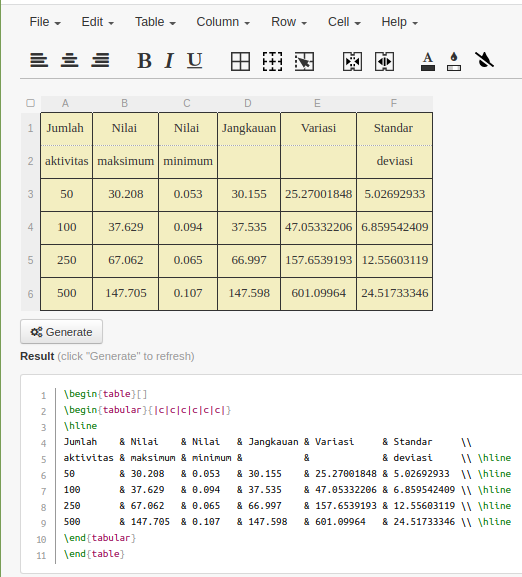
\includegraphics[width=0.5\textwidth]{assets/pics/tablesgenerator-dot-com.png}
% 	\caption{\textit{User interface} dari \textit{website} https://www.tablesgenerator.com/}
% 	\label{fig:tablesgenerator}
% \end{figure}

% Di sisi lain, tabel juga dapat diberi label dan caption seperti pada gambar.
% Caption pada tabel terletak pada bagian atas tabel.
% Contoh tabel sederhana dapat dilihat pada \tab~\ref{tab:tab1}.

% \begin{table}
% 	\centering
% 	\caption{Contoh Tabel}
% 	\label{tab:tab1}
% 	\begin{tabular}{| l | c r |}
% 		\hline
% 		        & kol 1 & kol 2 \\
% 		\hline
% 		baris 1 & 1     & 2     \\
% 		baris 2 & 3     & 4     \\
% 		baris 3 & 5     & 6     \\
% 		baris 4 & 7     & 8     \\
% 		baris 5 & 9     & 10    \\
% 		\hline
% 		jumlah  & 25    & 30    \\
% 		\hline
% 	\end{tabular}
% \end{table}

% Adapun untuk membuat tabel panjang yang bisa melebihi dari satu halaman, gunakan perintah \code{\bslash{}begin\{longtable\}} sebagai pengganti \code{\bslash{}begin\{table\}}. Di dalam \code{longtable} tidak perlu lagi ada \code{\bslash{}begin\{tabular\}}. Kemudian, tambahkan tanda \code{\bslash{}\bslash{}} setelah baris \code{\bslash{}label\{....\}}, agar tidak menimbulkan error saat menampilkan \f{caption} di bagian atas tabel. Kemudian, untuk membatasi header yang ingin diulang pada halaman-halaman berikutnya, gunakan perintah \code{\bslash{}endhead}. Contohnya adalah sebagai berikut:

% \begin{longtable}{| l | c r |}
% 	\caption{Contoh Tabel Panjang}
% 	\label{tab:tab2}         \\
% 	\hline
% 	         & kol 1 & kol 2 \\
% 	\hline
% 	\endfirsthead % batas akhir header yang akan muncul di halaman pertama
% 	\hline
% 	         & kol 1 & kol 2 \\
% 	\hline
% 	\endhead % batas akhir header yang akan muncul di halaman berikutnya
% 	baris 1  & 1     & 2     \\
% 	baris 2  & 3     & 4     \\
% 	baris 3  & 5     & 6     \\
% 	baris 4  & 7     & 8     \\
% 	baris 5  & 9     & 10    \\
% 	baris 6  & 11    & 12    \\
% 	baris 7  & 13    & 14    \\
% 	baris 8  & 15    & 16    \\
% 	baris 9  & 17    & 18    \\
% 	baris 10 & 19    & 20    \\
% 	baris 11 & 21    & 22    \\
% 	baris 12 & 23    & 24    \\
% 	baris 13 & 25    & 26    \\
% 	baris 14 & 27    & 28    \\
% 	baris 15 & 29    & 30    \\
% 	\hline
% \end{longtable}

% Ada jenis tabel lain yang dapat dibuat dengan \latex~berikut beberapa diantaranya.
% Contoh-contoh ini bersumber dari \url{http://en.wikibooks.org/wiki/LaTeX/Tables}

% \begin{table}
% 	\centering
% 	\caption{An Example of Rows Spanning Multiple Columns}
% 	\label{row.spanning}
% 	\begin{tabular}{|l|l|*{6}{c|}}
% 		\hline % create horizontal line
% 		No & Name & \multicolumn{3}{|c|}{Week 1} & \multicolumn{3}{|c|}{Week 2}                 \\
% 		\cline{3-8} % create line from 3rd column till 8th column
% 		   &      & A                            & B                            & C & A & B & C \\
% 		\hline
% 		1  & Lala & 1                            & 2                            & 3 & 4 & 5 & 6 \\
% 		2  & Lili & 1                            & 2                            & 3 & 4 & 5 & 6 \\
% 		3  & Lulu & 1                            & 2                            & 3 & 4 & 5 & 6 \\
% 		\hline
% 	\end{tabular}
% \end{table}

% \begin{table}
% 	\centering
% 	\caption{An Example of Columns Spanning Multiple Rows}
% 	\label{column.spanning}
% 	\begin{tabular}{|l|c|l|}
% 		\hline
% 		Percobaan               & Iterasi & Waktu    \\
% 		\hline
% 		Pertama                 & 1       & 0.1 sec  \\ \hline
% 		\multirow{2}{*}{Kedua}  & 1       & 0.1 sec  \\
% 		                        & 3       & 0.15 sec \\
% 		\hline
% 		\multirow{3}{*}{Ketiga} & 1       & 0.09 sec \\
% 		                        & 2       & 0.16 sec \\
% 		                        & 3       & 0.21 sec \\
% 		\hline
% 	\end{tabular}
% \end{table}

% \begin{table}
% 	\centering
% 	\caption{An Example of Spanning in Both Directions Simultaneously}
% 	\label{mix.spanning}
% 	\begin{tabular}{cc|c|c|c|c|}
% 		\cline{3-6}
% 		                                                &     & \multicolumn{4}{|c|}{Title}                 \\ \cline{3-6}
% 		                                                &     & A                           & B   & C   & D \\ \hline
% 		\multicolumn{1}{|c|}{\multirow{2}{*}{Type}}     &
% 		\multicolumn{1}{|c|}{X}                         & 1   & 2                           & 3   & 4       \\ \cline{2-6}
% 		\multicolumn{1}{|c|}{}                          &
% 		\multicolumn{1}{|c|}{Y}                         & 0.5 & 1.0                         & 1.5 & 2.0     \\ \cline{1-6}
% 		\multicolumn{1}{|c|}{\multirow{2}{*}{Resource}} &
% 		\multicolumn{1}{|c|}{I}                         & 10  & 20                          & 30  & 40      \\ \cline{2-6}
% 		\multicolumn{1}{|c|}{}                          &
% 		\multicolumn{1}{|c|}{J}                         & 5   & 10                          & 15  & 20      \\ \cline{1-6}
% 	\end{tabular}
% \end{table}


% %-----------------------------------------------------------------------------%
% \section{Keterkaitan Teori Dengan Penelitian}
% \label{sec:keterkaitan}
% %-----------------------------------------------------------------------------%
% \todo{Ada baiknya setelah menjelaskan teori-teori, Anda menjelaskan apa kaitan teori tersebut dengan penelitian Anda. Hal ini tentunya membantu pembaca dalam memahami bahwa teori yang Anda paparkan memang penting untuk memahami penelitian Anda nantinya.}

% \begin{figure}
% 	\centering
% 	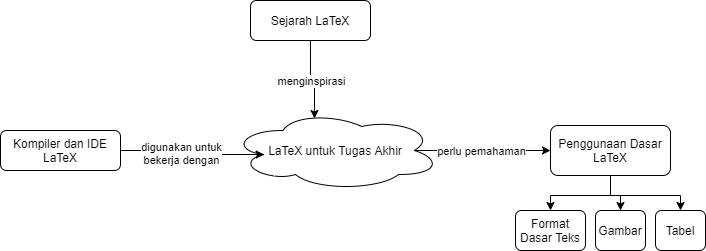
\includegraphics[width=\textwidth]{assets/pics/research_concept_map.png}
% 	\caption{Keterkaitan konsep hasil studi literatur terhadap penelitian}
% 	\label{fig:research_concept_map}
% \end{figure}

% \todo{Jelaskan \pic~\ref{fig:research_concept_map} di sini. Setiap gambar pada tugas akhir butuh penjelasan. Gambar hadir untuk mempermudah membaca memahami konteks, tetapi tidak bisa berdiri sendiri tanpa penjelasan. Terkait gambar, Anda juga bisa mengatur skalanya. Gambar kali ini lebarnya 0,8x dari lebar teks halaman.}
